\documentclass{article}
% PACKAGES %
\usepackage[english]{} % Sets the language
\usepackage[margin=2cm]{geometry} % Sets the margin size
\usepackage{fancyhdr} % Allows creation of headers
\usepackage{xcolor} % Allows the use of color in text
\usepackage{float} % Allows figures and tables to be floats
\usepackage{appendix}
\usepackage{amsmath} % Enhanced math package prepared by the American Mathematical Society
	\DeclareMathOperator{\sech}{sech} % Include sech
\usepackage{amssymb} % AMS symbols package
\usepackage{mathrsfs}% More math symbols
\usepackage{breqn} % Allows line breaking in math mode
\usepackage{cancel} % Allows math strikethroughs to show cancellations
\usepackage{bm} % Allows you to use \bm{} to make any symbol bold
\usepackage{bbold} % Allows more bold characters
\usepackage{verbatim} % Allows you to include code snippets
\usepackage{setspace} % Allows you to change the spacing between lines at different points in the document
\usepackage{parskip} % Allows you alter the spacing between paragraphs
\usepackage{multicol} % Allows text division into multiple columns
\usepackage{units} % Allows fractions to be expressed diagonally instead of vertically
\usepackage{booktabs,multirow,multirow} % Gives extra table functionality
\usepackage[final]{pdfpages} % Allows pdfs to be imported
\usepackage{hyperref} % Allows hyperlinks in the document
\usepackage{rotating} % Allows tables to be rotated
\usepackage{graphicx} % Enhanced package for including graphics/figures
	% Set path to figure image files
	\graphicspath{ {fig/} }
\usepackage{listings} % for including text files
	\lstset{basicstyle=\ttfamily\scriptsize,
        		  keywordstyle=\color{blue}\ttfamily,
        	  	  stringstyle=\color{red}\ttfamily,
          	  commentstyle=\color{gray}\ttfamily,
          	 }		
\newcommand{\tab}{\-\hspace{1cm}}

\newcommand{\Oh}{\hat{\Omega}}
\newcommand{\cur}{\bm{J}}
\newcommand{\rt}{(\bm{r},t)}
\newcommand{\rOt}{(\bm{r},\Oh,t)}


% Create a header w/ Name & Date
\pagestyle{fancy}
\rhead{\textbf{Mitch Negus} \; 9/22/2017}

\begin{document}
\thispagestyle{empty}

{\bf {\large {NE250 Homework {1} \hfill Mitch Negus\\
		\hspace*{\fill} 9/22/2017\\ }}}
		
%%%%%%%%%%%%%%%%%%%%%%%%%%%%%%%%%% PROBLEM 1 %%%%%%%%%%%%%%%%%%%%%%%%%%%%%%%%%%

\section*{Problem 1}

The number of molecules, $N$, found in a sample of a compound with mass $M$ is 
$$ N(\cdot) = \frac{M(\cdot) N_A}{m(\cdot)} $$
where $m$ is the molar mass of the compound, and $N_A$ is Avogadro's number ($N_A = 6.022 \times 10^{23}$ molecules per mole). Where each actinide isotope is found only once in a molecule of its respective oxide, $N$ also gives the number of atoms of an isotope in the sample. 

To find $N$, we begin by finding the masses of the compounds in the fuel. We can decompose the total mass of the fuel, $M_f$, into its mixed oxide components:
$$ M_f = M(\text{UO}_2) + M(\text{PuO}_2). $$
Given a weight percent for plutonium, $w_{\text{P}}$, we note that $w_{\text{U}} = 1-w_{\text{P}}$ and so calculate the total masses of both the UO$_2$ and the PuO$_2$ to be
$$ M(\text{UO}_2) = (1-w_{\text{P}})M_f	$$
$$ M(\text{PuO}_2) = w_{\text{P}}M_f. $$

We are told that the uranium is all $^{238}$U, so 
$$ M(^{238}\text{UO}_2) = M(\text{UO}_2) = (1-w_{\text{P}})M_f. $$

<<<<<<< HEAD
The weight percents of the plutonium isotope oxides are also given (as a fraction of total plutonium oxide). Using $^{239}\text{PuO}_2$ as an example
$$ M(^{239}\text{PuO}_2) = w_{\text{P}9}M(\text{PuO}_2) = w_{\text{P}9}w_{\text{P}}M_f. $$


Next, we must determine the molar masses of the various oxides. For uranium,
$$ m(^{238}\text{UO}_2) = m(^{238}\text{U}) + 2m(\text{O}), $$
and similarly for plutonium.

When we combine the total and molar masses to determine the total number of atoms for each isotope, we find:\\
\tab 6.69$\times 10^{20} \text{ atoms of }^{238}$U	\\
\tab 4.65$\times 10^{20} \text{ atoms of }^{239}$Pu	\\
\tab 1.45$\times 10^{20} \text{ atoms of }^{240}$Pu	\\
\tab 3.84$\times 10^{19} \text{ atoms of }^{241}$Pu	\\
\tab 1.78$\times 10^{19} \text{ atoms of }^{242}$Pu	\\

(for full calculation, see Jupyter notebook, attached)

%%%%%%%%%%%%%%%%%%%%%%%%%%%%%%%%%% PROBLEM 2 %%%%%%%%%%%%%%%%%%%%%%%%%%%%%%%%%%

\section*{Problem 2}

The mean free path of a particle is given by the formula
$$ \lambda = \frac{1}{\Sigma_t} $$

when scattering is considered to be isotropic. The macroscopic scattering cross section can be reexpressed in terms of the number density of the material, $n$, and the microscopic cross section, $\sigma_t$. For mixtures, the macroscopic cross section is the sum of the macroscopic cross sections of its components.
$$ \Sigma_{t,\text{mix}} = \sum_i \Sigma_{t,i} = \sum_i n_i \sigma_i $$

Additionally, the number density of the material can be found from the material density, $\rho$, the molar mass of the material, $m$, and Avogadro's number.
$$ n = \frac{\rho_i N_A}{m_i} $$

Then the mean free path is
$$ \lambda = \frac{1}{\sum_i \frac{\rho_i N_A \sigma_{t,i}}{m_i}} $$

NIST gives the composition of air as 75.5\% nitrogen, 23.1\% oxygen, and 1.3\% argon by mass. We will assume that the nitrogen is entirely $^{14}$N, oxygen is entirely $^{16}$O, and $^{40}$Ar, which comprise more than 99.5\% of their respective element naturally. Water is 11.2\% hydrogen and 88.8\% oxygen by mass. We are assuming the hydrogen is entirely $^{1}$H and the oxygen is entirely $^{16}$O. According to the World Nuclear Association, natural uranium is 99.3\% U238 and 0.7\% U235 by mass. Using these values in the equation for mean free path, we find the following results:

\begin{multicols}{3}

\subsection*{\textit{a.}) \small 14 MeV neutrons}
Mean Free Path in\\
	\tab air:  $\lambda = 12773.78$ cm\\
	\tab water:  $\lambda = 10.08$ cm\\
	\tab uranium:  $\lambda = 3.53$ cm\\

\subsection*{\textit{b.}) \small 1 MeV neutrons}
Mean Free Path in\\
	\tab air:  $\lambda = 5643.26$ cm\\
	\tab water:  $\lambda = 1.8$ cm\\
	\tab uranium:  $\lambda = 2.93$ cm\\

\subsection*{\textit{c.}) \small 0.05 eV neutrons}
Mean Free Path in\\
	\tab air:  $\lambda = 2086.21$ cm\\
	\tab water:  $\lambda = 0.66$ cm\\
	\tab uranium:  $\lambda = 1.57$ cm\\

\end{multicols}




%%%%%%%%%%%%%%%%%%%%%%%%%%%%%%%%%% PROBLEM 3 %%%%%%%%%%%%%%%%%%%%%%%%%%%%%%%%%%

\section*{Problem 3}

Cross sections plotted using ENDF/B-VII.1 from \href{http://atom.kaeri.re.kr/nuchart/}{KAERI}.

\begin{multicols}{2}
\tab\textbf{Fission Cross Sections}\\
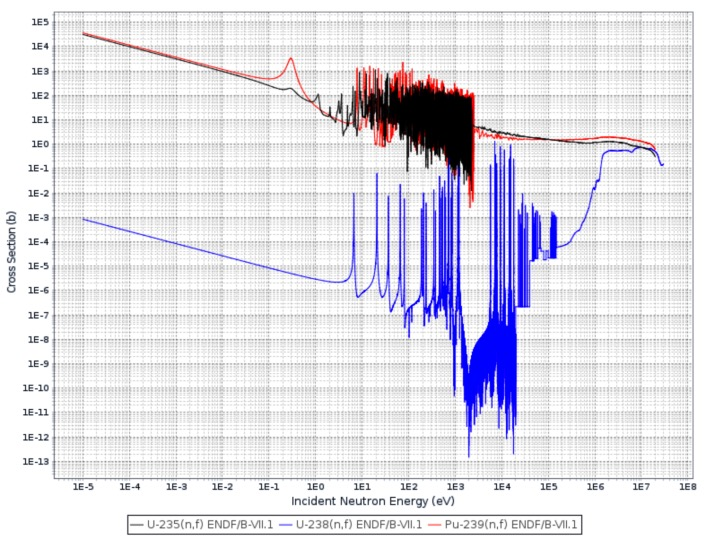
\includegraphics[width=9cm]{fission_xs}

\tab\textbf{Capture Cross Sections}\\
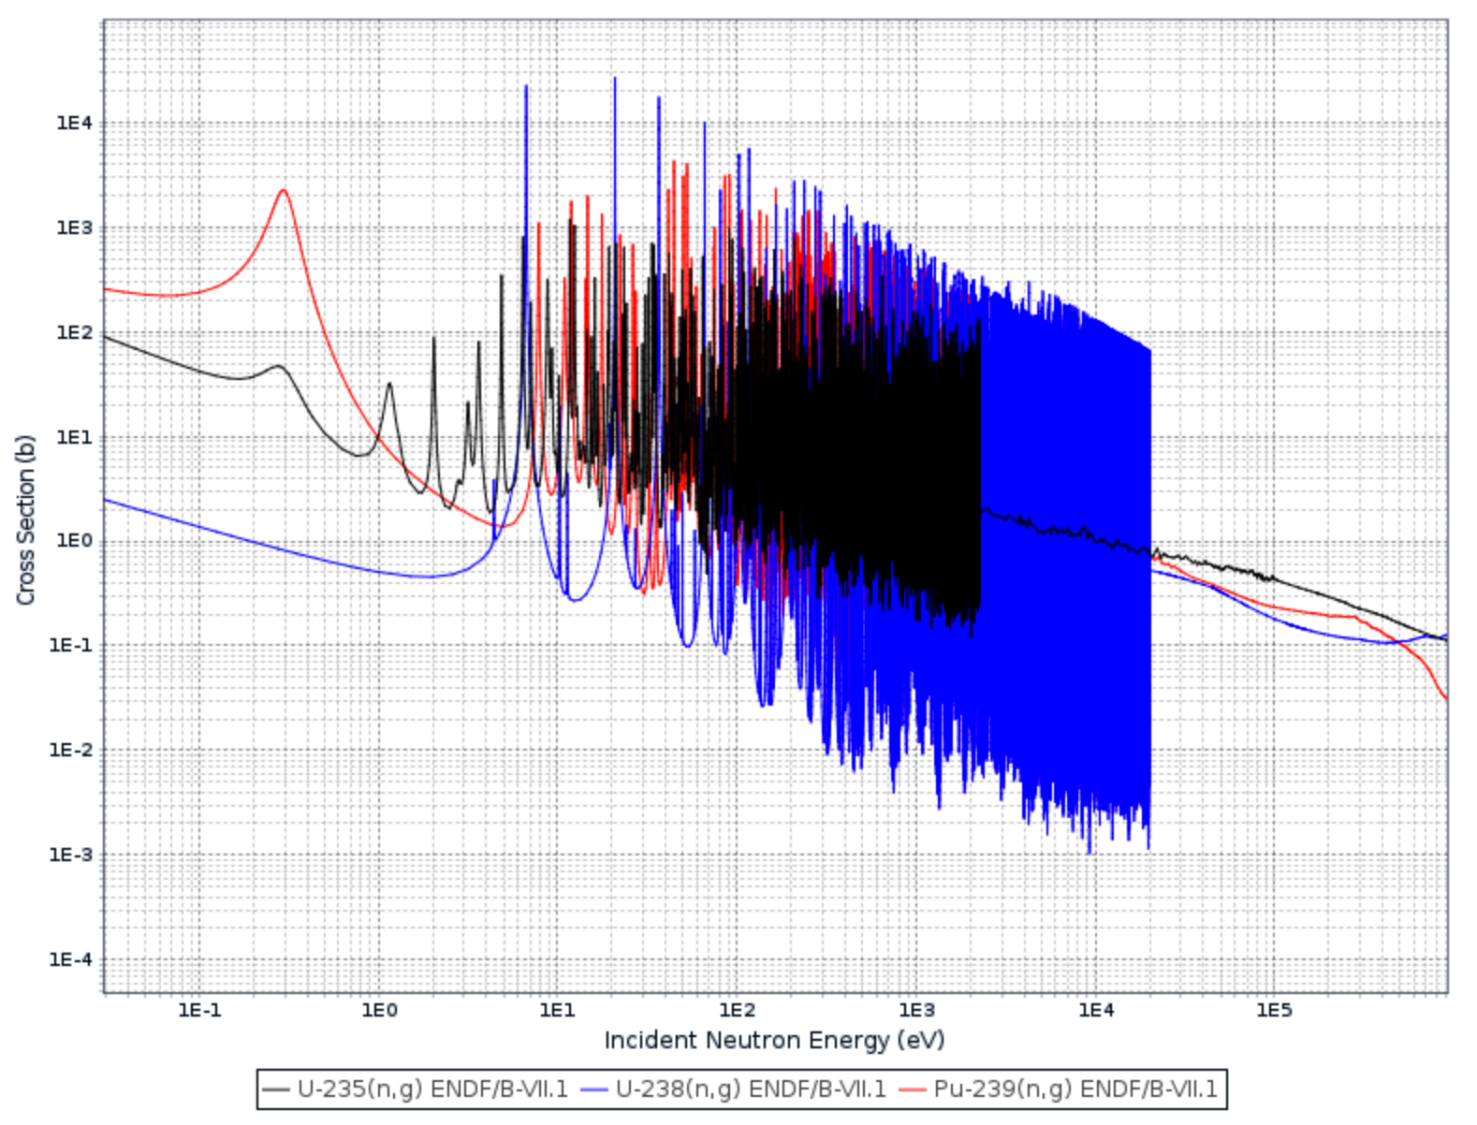
\includegraphics[width=9cm]{capture_xs}
\end{multicols}

Capture-to-fission ratios at:
\begin{multicols}{2}
\begin{onehalfspace}
\textbf{0.0253 eV}\\
$^{238}\text{U}$: \tab $\frac{3\text{ b}}{0.00003\text{ b}} = 100000$\\
$^{239}\text{Pu}$: \tab $\frac{300\text{ b}}{800\text{ b}} = 0.38$\\
$^{235}\text{U}$: \tab $\frac{100\text{ b}}{700\text{ b}} = 0.14$\\
\textbf{0.73 MeV}\\
$^{238}\text{U}$: \tab $\frac{0.13\text{ b}}{0.004\text{ b}} = 32.5$\\
$^{235}\text{U}$: \tab $\frac{0.13\text{ b}}{1\text{ b}} = 0.13$\\
$^{239}\text{Pu}$: \tab $\frac{0.07\text{ b}}{2\text{ b}} = 0.04$
\end{onehalfspace}
\end{multicols}



%%%%%%%%%%%%%%%%%%%%%%%%%%%%%%%%%% PROBLEM 4 %%%%%%%%%%%%%%%%%%%%%%%%%%%%%%%%%%

\section*{Problem 4}

The most prevalent, stable isotopes of natural boron are $^{10}$B and $^{11}$B. Similarly, natural gadolinium mostly contains the isotopes $^{154}$Gd, $^{155}$Gd, $^{156}$Gd, $^{157}$Gd, $^{158}$Gd, and $^{160}$Gd.

For the isotopes of both boron and gadolinium, neutron absorption occur primarily through $(n,\gamma),(n,\alpha)$, or $(n,p)$ reactions. Cross sections for absorption modes in the most common natural isotopes of boron (left) and gadolinium (right) are shown below.

\begin{multicols}{2}
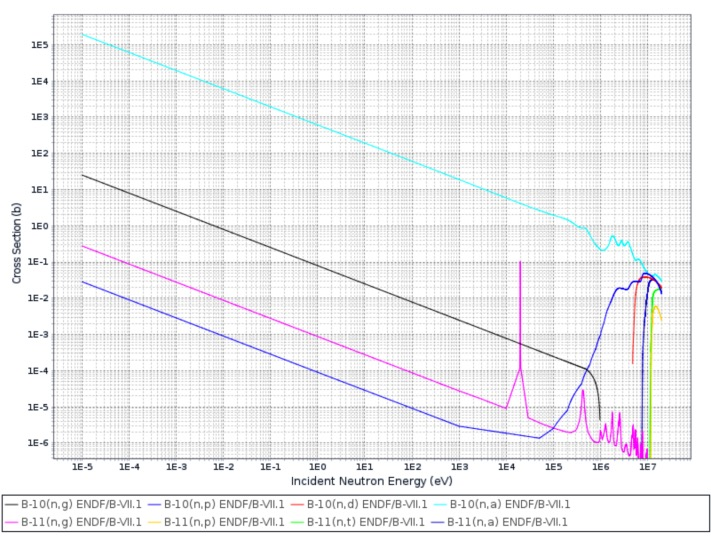
\includegraphics[width=8cm]{B_xs_abs}
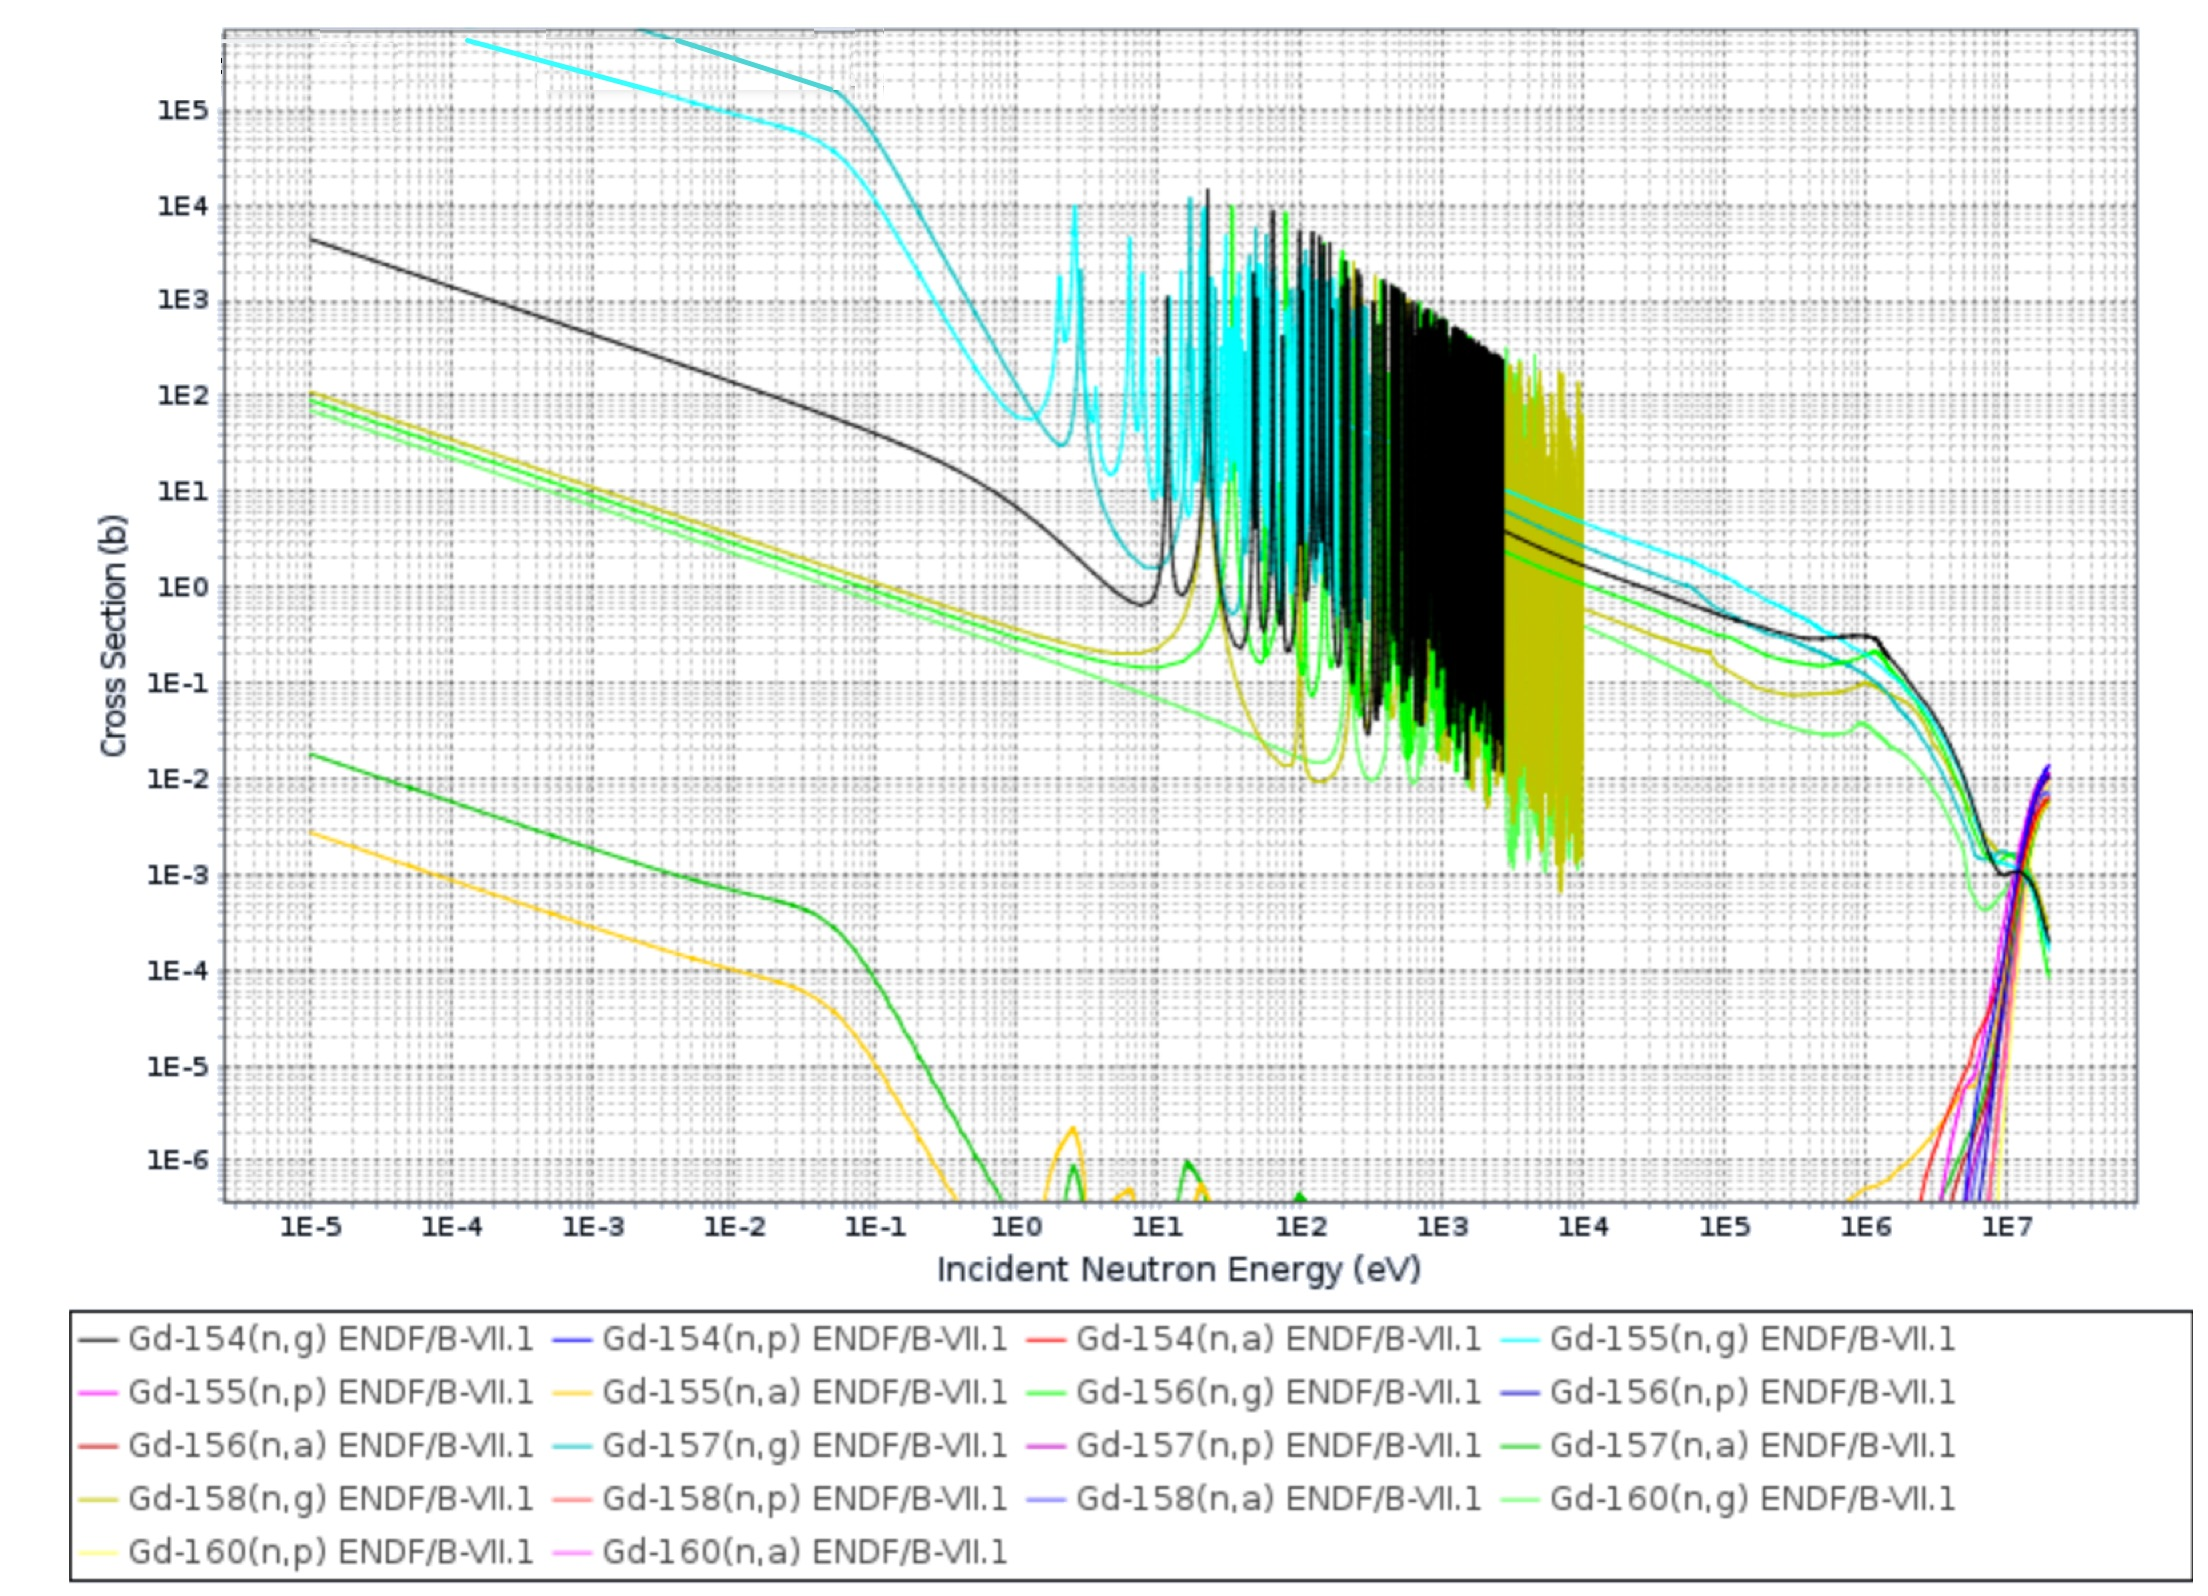
\includegraphics[width=8cm]{Gd_xs_abs}
\end{multicols}

At thermal energies, the following isotopes and reactions are most absorbing:\\
$^{10}$B, $(n,\alpha)$; $^{155}$Gd, $(n,\gamma)$; $^{157}$$, (n,\gamma)$\\



%%%%%%%%%%%%%%%%%%%%%%%%%%%%%%%%%% PROBLEM 5 %%%%%%%%%%%%%%%%%%%%%%%%%%%%%%%%%%

\section*{Problem 5}

The required thermal power density is 400kW/liter. In terms of energy, this is 
$$ \frac{400\text{ kW}}{\text{liter}} \cdot \frac{1000 \text{ J/s}}{\text{kW}} \cdot \frac{1 \text{ eV}}{1.60 \times 10^{-19} \text{ J}} = \frac{2.50 \times 10^{24} \text{ eV}}{\text{s} \cdot \text{liter}} $$

The energy that can be harnessed from the fission of $^{239}$Pu is $198.5 \pm 0.8$ MeV (Duderstadt \& Hamilton, Table 2-5). At a rate of 198.5 MeV/fission, the fission rate density is 
$$ \frac{2.50 \times 10^{24} \text{ eV}}{\text{s} \cdot \text{liter}} \cdot \frac{\text{fission}}{198.5 \times 10^6 \text{ eV}} = \frac{1.26 \times 10^{16} \text{ fissions}}{\text{s} \cdot \text{liter}} $$

$$\boxed{ 1.26 \times 10^{13} \text{ fissions} \cdot \text{s}^{-1} \cdot \text{cm}^{-3} }$$



%%%%%%%%%%%%%%%%%%%%%%%%%%%%%%%%%% PROBLEM 6 %%%%%%%%%%%%%%%%%%%%%%%%%%%%%%%%%%

\section*{Problem 6}

A detector with 50\% efficiency measuring 346,573 CPM is analyzing a sample that is emitting at 693,146 CPM. If this sample is $^{116}$In with $T_{1/2} = 54$ min, we can use the definition of activity $\mathcal{A} = \lambda N(t)$ to determine the initial number of $^{116}$In nuclei. 
$$ \mathcal{A_0} = 693146 \text{ CPM} = \lambda N_0 $$
Also, $\lambda = \frac{\ln 2}{T_{1/2}}$, so $\lambda = 0.01284$ min$^{-1}$ and
$$ N_0 = \frac{693146\text{ CPM}}{0.01284\text{ min}^{-1}} $$
$$ N_0 = 5.4 \times 10^7 \text{ nuclei} $$
The rule for radioactive decay states that the number of nuclei remaining from an initial sample of $N_0$ nuclei at time $t$ can be approximated by
$$ N(t) = N_0 e^{-\lambda t} $$
Taking the derivative of this function, we find that the rate of change is 
$$ R(t) = -\lambda N_0 e^{-\lambda t} $$
If we negate the rate of change and multiply by the time $dt$ we arrive at an expression for the number of nuclei decaying in the time period of $t$ to $dt$. Then, if we divide this by the initial count of nuclei, we get the probability that a given nuclei will decay in time $t$ to $t+dt$. 
$$ p(t)dt = \lambda e^{-\lambda t} dt $$
If we integrate this equation over a time interval, we can find the total probability that a nucleus will decay in that interval.
\begin{align*}
P_d(t) = \int_0^t p(t')dt'	&= \int_0^t \lambda e^{-\lambda t'} dt'\\
							&= \lambda \int_0^t e^{-\lambda t'} dt'\\
							&= \lambda \left[ -\frac{1}{\lambda} e^{-\lambda t'} \right]_0^T\\
							&= 1 - e^{-\lambda t} \\
\end{align*}
From 4:00pm Tuesday to 2:00pm Thursday is 46 hours, or 2760 minutes. The probability for a given nucleus to decay in that time is
\begin{align*}
P_d(2760\text{ min})	&= 1-e^{-(0.01284 \text{ min}^{-1})(2760\text{ min})} \\ 
					&= 1-e^{-35.44} \\
\end{align*}
This is the probability that one nucleus decays. The probability that all nuclei decay is the product of the probabilities for each nuclei.
\begin{align*} 
P_{N_0}(t)					&= (1 - e^{-\lambda t})^{N_0} \\
P_{N_0}(2760\text{ min})	&= (1- e^{-35.44})^{5.4\times10^7} \\
\end {align*}
The probability that no nuclei of the radioactive In sample remain is 0.999999978072...
%%% ???If we note that $\ln(1-x) \approx -x$ when $x \ll 1$, we find
%%% $$ \ln\left[P(2760\text{ min})\right] = \ln\left[(1-e^{-35.44})^{5.4\times10^7}\right] \approx e^{-35.44} $$



%%%%%%%%%%%%%%%%%%%%%%%%%%%%%%%%%% PROBLEM 8 %%%%%%%%%%%%%%%%%%%%%%%%%%%%%%%%%%

\section*{Problem 8}

We can calculate a theoretical maximum of the multiplication factor by looking at the definition of the multiplication factor:
$$ k = \frac{\text{ \# neutrons in generation}i+1}{\text{ \# neutrons in generation} i}. $$
This equation can be maximized if no losses occur between generations, and every neutron produces a fission event. If this is the case, then each of $N$ neutrons in generation $i$ produces $\nu N$ neutrons in generation $i+1$ through fission (assuming we have sufficiently many fissionable nuclei for the average number of neutrons produced per fission, $\nu$, to be accurate).

Then, it can be determined that the the maximum theoretical multiplication factor is 
$$ k = \frac{\nu N}{N} $$
$$\boxed{ k = \nu }$$



%%%%%%%%%%%%%%%%%%%%%%%%%%%%%%%%%% PROBLEM 9 %%%%%%%%%%%%%%%%%%%%%%%%%%%%%%%%%%

\section*{Problem 9}

\textbf{\textit{a.})} If rapidly compressed to half volume, the reactor's density will dramatically increase. Cross sections vary directly with density, and so the reactor's cross sections will also increase. Greater cross sections mean more chances for fission to be induced, and the multiplication factor will rise. A critical reactor would then become \underline{supercritical}.

\textbf{\textit{b.})} If squashed into an ellipsoidal shape, the reactor's surface area would increase, with no change in volume. Greater surface area means that more neutrons would leak from the reactor, and the critical reactor would become \underline{subcritical} (the streaming term in the TE will grow, $k$ must decrease).

\textbf{\textit{c.})} Wrapping a sheet of cadmium around the outside of the reactor will cause neutrons to be reflected back into the reactor volume (assuming it replaces void). This will increase the neutrons able to cause fission, and the reactor will become \underline{supercritcal}  (the streaming term in the TE will diminish, $k$ must increase).

\textbf{\textit{d.})} Again, neutrons will be reflected back into the reactor. A greater neutron density increases the neutron flux and rate of fission. The multiplication factor will increase and the reactor will become \underline{supercritical}  (the streaming term in the TE will diminish, $k$ must increase).

\textbf{\textit{e.})} Adding an external neutron source to the reactor will also trigger an increase in the multiplication factor. There will be more neutrons in the system to cause fission events.

\textbf{\textit{f.})} Placing an identical reactor nearby the original could be considered as if adding another source. As in that case, the multiplication factor will increase.

\textbf{\textit{g.})} Over time, the fissionable nuclei in the reactor will be consumed in the fission reaction. With less fissionable nuclei, the fission cross sections of the reactor fuel material will decrease. The reactor will become \underline{subcritical} and the multiplication factor will decrease.



%%%%%%%%%%%%%%%%%%%%%%%%%%%%%%%%%% PROBLEM 10 %%%%%%%%%%%%%%%%%%%%%%%%%%%%%%%%%%

\section*{Problem 10}

\textbf{Assumptions of the neutron transport equation:}
\begin{enumerate}
	\item \textit{Neutrons are pointlike.} A reasonable assumption because the de Broglie wavelength of a neutron is significantlly less than the diameter of an atom. This assumption allows us to neglect rotation and quantum effects and write the transport equation as a function of energy. We need only being concerned with the particle's translational kinetic energy.
	\item \textit{Neutral particles travel in straight lines.} Neutron trajectories will not bend between collisions, and we can make the assumption that $\frac{\partial \theta}{\partial t} = 0$ and $\frac{\partial \varphi}{\partial t} = 0$.
	\item \textit{Particle-particle collisions are negligible.} Neutrons are generally very unlikely to collide/otherwise interact with other neutrons, allowing us to express the transport equation as a linear differential equation.
	\item \textit{Material properties are isotropic.} Valid when neutrons are moving with an appreciable velocity, this condition allows us to establish cross sections simply as functions of $\vec{r}$ and $E$ (not $\Oh$).
	\item \textit{Material composition is independent of time.} Similar to assumption 5, our cross sections become dependent only on $\vec{r}$ and $E$. Though material does change over long time scales (\textit{i.e.} burnup) this assumption is valid for short term neutronics calculations.
	\item \textit{Quantities are expected values.} We may be unable to properly predict fluctuations in our results for cases where we are dealing with low density media.

\end{enumerate}



%%%%%%%%%%%%%%%%%%%%%%%%%%%%%%%%%% PROBLEM 11 %%%%%%%%%%%%%%%%%%%%%%%%%%%%%%%%%%

\section*{Problem 11}

To model the neutron transport in a one-dimensional rod, we follow the same procedure as for a three-dimensional volume with some adjustments.

Before starting, we must replace the volume considered by the 3D case by a 1D length, $L$. 

\textbf{Time-rate-of-change}\\
First we consider the rate of change of particles in the rod. This is accomplished by taking the derivative of the neutron population with respect to time at a location, and then integrating that over the length of the rod.
$$ \int_L \frac{\partial}{\partial t}n(x,E,\Oh,t)dx\,d\Oh\,dE $$
It should be noted here that in one dimension, the direction of the particle ($\Oh$) can only be in the positive or negative direction. With this finite domain, it is easy to express the neutron population as
$$ n(x,E,\Oh,t)\,d\Oh = n_{+}(x,E,t) + n_{-}(x,E,t). $$
Then, the time-rate-of-change becomes
$$ \int_L \frac{\partial}{\partial t}\left[n_{+}(x,E,t) + n_{-}(x,E,t)\right]dx\,dE $$

\textbf{Scattering}\\
For the scattering, we consider all scattering events that can take place in length $L$ over the full range of energies (these are the two integrals). Then, we turn what had been an integral over the resulting angle into a discrete sum of the two directions into which the particle could be scattered. Again, we include the neutron density as it's two directional components.
$$ \int_L \int_0^{\infty} \left[\Sigma_s^{+}(E'\rightarrow E) + \Sigma_s^{-}(E'\rightarrow E)\right] v' \left[n_{+}(x,E',t) + n_{-}(x,E',t)\right]dx\,dE'\,dE$$

\textbf{Fission}\\
Now we can consider fission. Whereas before isotropic production of fission neutrons resulted in a rate of $\frac{1}{4\pi}$ per steradian, we now have a $\frac{1}{2}$ chance that neutrons are produced in either the left or right directions. The fission term is then
$$ \frac{\chi(E)}{2} \int_L \int_0^{\infty} \nu(E') \Sigma_f(E') v' \left[n_{+}(x,E',t) + n_{-}(x,E',t)\right]dx\,dE'\,dE $$

\textbf{Source}\\
Like the neutron population, the source term can be divided into its two components (left and right), rather than a continuous distribution over angle. Integrating over the rod gives
$$ \int_L \left[s_{+}(x,E,t) + s_{-}(x,E,t)\right]dx\,dE $$

\textbf{Absorption}\\
Collisions of the neutron may cause it to be absorbed or scattered.
$$ \int_L \Sigma_t v \left[n_{+}(x,E,t) + n_{-}(x,E,t)\right]dx\,dE $$

\textbf{Streaming}\\
Like in the 3D case, we can define $\vec{j}$ as the expected number of particles exiting the 1D rod. Since we only need to account for particles entering or leaving in the single dimension, the integral over surface $S$ becomes unnecessary, and can be replaced by the current at both ends of the rod. We retain the integral (now over $L$) for reasons apparent later, but incorporate this fact through a delta function.
$$ \int_L \left[\vec{j}(x,E,\Oh,t)\delta(\frac{L}{2}) + \vec{j}(x,E,\Oh,t)\delta(-\frac{L}{2})\right]dx\,dE\,d\Oh $$
Also, we can eliminate the $\Oh$ dependence since we no longer need to account for particles traveling in 3D. Instead, we can divide our equation up again into the two components, one for particles traveling left and another for particles traveling right at each boundary. The result of these operations is
$$ \int_L \left[j_{+}(x,E,t)\delta(x-\frac{L}{2}) + j_{-}(x,E,t)\delta(x-\frac{L}{2}) + j_{+}(x,E,t)\delta(x+\frac{L}{2}) + j_{-}(x,E,t)\delta(x+\frac{L}{2})\right]dx\,dE $$
Noting that $j_{\pm} = vn_{\pm}$,
$$ \int_L v \left[n_{+}(x,E,t)\delta(x-\frac{L}{2}) + n_{-}(x,E,t)\delta(x-\frac{L}{2}) + n_{+}(x,E,t)\delta(x+\frac{L}{2}) + n_{-}(x,E,t)\delta(x+\frac{L}{2})\right]dx\,dE $$

The full 1D transport equation is then (canceling $dE$ in all terms, and forming one integral over $L$)
\begin{dmath*}
\int_L \Bigg[ \frac{\partial}{\partial t} \left[n_{+}(x,E,t) + n_{-}(x,E,t)\right] + \Sigma_t v \left[n_{+}(x,E,t) + n_{-}(x,E,t)\right] + v \left[n_{+}(x,E,t)\delta(x-\frac{L}{2}) + n_{-}(x,E,t)\delta(x-\frac{L}{2}) + n_{+}(x,E,t)\delta(x+\frac{L}{2}) + n_{-}(x,E,t)\delta(x+\frac{L}{2})\right] - \int_0^{\infty} \left[\Sigma_s^{+}(E'\rightarrow E) + \Sigma_s^{-}(E'\rightarrow E)\right] v' \left[n_{+}(x,E',t) + n_{-}(x,E',t)\right]dE' - \left[s_{+}(x,E,t) + s_{-}(x,E,t)\right] - \frac{\chi(E)}{2} \int_0^{\infty} \nu(E') \Sigma_f(E') v' \left[n_{+}(x,E',t) + n_{-}(x,E',t)\right]dE'  \Bigg]dx = 0
\end{dmath*}
Now since, for $\int_L f(x)\,dx = 0, f(x) = 0$, we can say that the integrand of the integral over $L$ is equal to zero. Also, the product
$$f(x)\delta(x-a) = \begin{cases} 	f(a) 	& x=a\\
									0		& \text{otherwise}
\end{cases}$$
so then
\begin{dmath*}
\frac{\partial}{\partial t} \left[n_{+}(x,E,t) + n_{-}(x,E,t)\right] + \Sigma_t v \left[n_{+}(x,E,t) + n_{-}(x,E,t)\right] + v \left[n_{+}(\frac{L}{2},E,t) + n_{-}(\frac{L}{2},E,t) + n_{+}(-\frac{L}{2},E,t) + n_{-}(-\frac{L}{2},E,t)\right] - \int_0^{\infty} \left[\Sigma_s^{+}(E'\rightarrow E) + \Sigma_s^{-}(E'\rightarrow E)\right] v' \left[n_{+}(x,E',t) + n_{-}(x,E',t)\right]dE' - \left[s_{+}(x,E,t) + s_{-}(x,E,t)\right] - \frac{\chi(E)}{2} \int_0^{\infty} \nu(E') \Sigma_f(E') v' \left[n_{+}(x,E',t) + n_{-}(x,E',t)\right]dE' = 0
\end{dmath*}


\subsection*{\textit{b.})}

If we make a one speed approximation, we can state that cross sections are generally independent. We can also conclude that $\Sigma_{s}^{\pm}(E' \rightarrow E) = \Sigma_{s}^{\pm}\delta(E' \rightarrow E)$. Our 1D-rod transport equation simplifies to
\begin{dmath*}
\frac{\partial}{\partial t} \left[n_{+}(x,t) + n_{-}(x,t)\right] + \Sigma_t v \left[n_{+}(x,t) + n_{-}(x,t)\right] + v \left[n_{+}(\frac{L}{2},t) + n_{-}(\frac{L}{2},t) + n_{+}(-\frac{L}{2},t) + n_{-}(-\frac{L}{2},t)\right] - (\Sigma_s^{+} + \Sigma_s^{-}) v \left[n_{+}(x,t) + n_{-}(x,t)\right] - \left[s_{+}(x,t) + s_{-}(x,t)\right] - \frac{\chi}{2} \nu \Sigma_f v \left[n_{+}(x,t) + n_{-}(x,t)\right] = 0
\end{dmath*}

\subsection*{\textit{c.})}
The initial condition for our (one speed) system is simply that $n_+(x,0)=n_{+,0}(x)$ and $n_-(x,0)=n_{-,0}(x)$ and our boundary conditions are that $n_-(\frac{L}{2},t)=0$ and $n_+(-\frac{L}{2},t)=0$ assuming that neutrons do not reenter the system. 



%%%%%%%%%%%%%%%%%%%%%%%%%%%%%%%%%% PROBLEM 12 %%%%%%%%%%%%%%%%%%%%%%%%%%%%%%%%%%

\section*{Problem 12}

\subsection*{\textit{a.})}

We can find $\phi(z)$ by integrating the given equation 
$$ \varphi(z,\mu) = \phi_0 \left[\cos(Bz) + A \mu \sin(Bz)\right] $$
over all $\mu$
\begin{align*}
\phi(z)	&= 2\pi \int_{-1}^{1} \phi(z,\mu) d\mu \\
		&= 2\pi \int_{-1}^{1} \phi_0\left[\cos(Bz) + A \mu \sin(Bz)\right] d\mu \\
		&= 2\pi \cos(Bz) \int_{-1}^{1} d\mu + \phi_0 A \sin(Bz) \int_{-1}^{1} \mu d\mu\\
		&= 2\pi \cos(Bz) (2) + \bcancel{\phi_0 A \sin(Bz) \left[ \frac{\mu^2}{2} \right]_{-1}^{1}}_{\;0}\\
\phi(z)	&= 4\pi \cos(Bz)
\end{align*}
According to diffusion theory, $J(z) = -D \nabla \phi(z)$. In 1D, the gradient takes the form of a single derivative, $\nabla = \frac{d}{dz}$. By definition 
$$ J(z) = \int_{4\pi} d\Oh \, \Oh \varphi(z,\mu).$$
We can substitute 
\begin{align*}
J(z)	&= 2\pi \int_{-1}^{1} \mu \, \varphi(z,\mu) \, d\mu \\
		&= 2\pi \int_{-1}^{1} \mu \, \phi_0 \left[\cos(Bz) + A \mu \sin(Bz)\right] \, d\mu \\
		&= 2\pi\phi_0 \left( \int_{-1}^{1} \mu \, \cos(Bz) \, d\mu + \int_{-1}^{1} A \mu^2 \sin(Bz) \, d\mu \right) \\
		&= 2\pi\phi_0 \left( \cos(Bz) \left[\frac{\mu^2}{2} \right]_{-1}^{1} + A \sin(Bz) \left[ \frac{\mu^3}{3} \right]_{-1}^{1} \right) \\
		&= 2\pi\phi_0 \left( 0 + \frac{2A\sin(Bz)}{3} \right) \\
J(z)	&= \frac{4\pi\phi_0A\sin(Bz)}{3}
\end{align*}


\subsection*{\textit{b.})}

If we now note that $A = \frac{3J(z)}{4\pi\phi_0\sin(Bz)}$, then we can rewrite our original equation for $\varphi$ in terms of $\phi(z)$ and $J(z)$.
\begin{align*}
\varphi(z,\mu)	&= \phi_0 \left[\cos(Bz) + A \mu \sin(Bz)\right] \\
				&= \phi_0 \left[\cos(Bz) + \left(\frac{3J(z)}{4\pi\phi_0\sin(Bz)}\right) \mu \sin(Bz)\right]\\
\varphi(z,\mu)	&= \frac{\phi_0}{4\pi} + \frac{3J(z)\mu}{4\pi}
\end{align*}


\subsection*{\textit{c.})}

Next, we must calculate $J_{+}(z)$ and $J_{-}(z)$. Again, by definition
$$ J_{\pm}(z) = 2\pi \int_0^{\pm1} \mu \, \varphi(z,\mu) \, d\mu .$$
Solving, we find
\begin{align*}
J_{\pm}(z)	&= 2\pi \int_0^{\pm1} \mu \, \varphi(z,\mu) \, d\mu \\
			&= 2\pi \int_0^{\pm1} \mu \, \phi_0 \left[\cos(Bz) + A \mu \sin(Bz)\right] \, d\mu \\
			&= 2\pi\phi_0 \left[ \int_0^{\pm1} \mu \, \cos(Bz) \, d\mu + \int_0^{\pm1} A \mu^2 \sin(Bz) \, d\mu \right] \\ 
			&= 2\pi\phi_0 \left[ \cos(Bz) \int_0^{\pm1} \mu \, d\mu + A \sin(Bz) \int_0^{\pm1} \mu^2 \, d\mu \right] \\ 
			&= 2\pi\phi_0 \left[ \cos(Bz) \left[ \frac{\mu^2}{2} \right]_0^{\pm1} + A \sin(Bz) \left[ \frac{\mu^3}{3} \right]_0^{\pm1} \right] \\ 
			&= 2\pi\phi_0 \left[ \frac{\cos(Bz)}{2} \pm \frac{A \sin(Bz)}{3} \right] \\
J_{\pm}(z)	&= \pi\phi_0\cos(Bz) \pm \frac{2\pi\phi_0 A \sin(Bz)}{3} \\ 
\end{align*}


\subsection*{\textit{d.})}

We can check our results by subtracting $J_{+}(z)$ and $J_{-}(z)$ and showing that their difference is $J(z)$. 
\begin{align*}
J_{+}(z) - J_{-}(z)	&= \left(\pi\phi_0\cos(Bz) + \frac{2\pi\phi_0 A \sin(Bz)}{3}\right) - \left(\pi\phi_0\cos(Bz) - \frac{2\pi\phi_0 A \sin(Bz)}{3}\right) \\
					&= \pi\phi_0\cos(Bz) + \frac{2\pi\phi_0 A \sin(Bz)}{3} - \pi\phi_0\cos(Bz) + \frac{2\pi\phi_0 A \sin(Bz)}{3} \\
J_{+}(z) - J_{-}(z)	&= \frac{4\pi\phi_0 A \sin(Bz)}{3} = J(z)
\end{align*}



%%%%%%%%%%%%%%%%%%%%%%%%%%%%%%%%%% PROBLEM 13 %%%%%%%%%%%%%%%%%%%%%%%%%%%%%%%%%%

Diffusion theory is built upon the assumption that the angular flux can be adequately represented by a linearly anisotropic angular dependence. This assumption can be formulated as
$$\psi\rOt \approx \frac{\phi\rt}{4\pi} + \frac{3\cur\rt}{4\pi}\cdot \Oh$$

Now, we can start with the definition of partial current,
$$ J_{\pm} = \int_{2\pi\pm} d\Oh \, \hat{e}_s \cdot \bm{j}\rOt .$$
and reduce it to being solely in terms of $\phi$. First, we note that $\bm{j}\rOt = \psi\rOt$, so
$$ J_{\pm} = \int_{2\pi\pm} d\Oh \, \hat{e}_s \cdot \Oh \, \psi\rOt $$
Now, if we substitute the assumption for $\psi$ above, this can be reexpressed as
$$ J_{\pm} \approx \int_{2\pi\pm} d\Oh \, \hat{e}_s \cdot \Oh \, \left(\frac{\phi\rt}{4\pi} + \frac{3\cur\rt}{4\pi}\cdot \Oh\right) .$$
We simplify this equation
\begin{align*}
J_{\pm}	&\approx \int_{2\pi\pm} d\Oh \, \hat{e}_s \cdot \Oh \, \left(\frac{\phi\rt}{4\pi} + \frac{3\cur\rt}{4\pi}\cdot \Oh\right) \\
		&\approx \int_{2\pi\pm} d\Oh \, \hat{e}_s \cdot \Oh \, \frac{\phi\rt}{4\pi} + \int_{2\pi\pm} d\Oh \, \hat{e}_s \cdot \Oh \frac{3\cur\rt}{4\pi}\cdot \Oh \\
		&\approx \frac{\phi\rt}{4\pi} \int_{2\pi\pm} d\Oh \, \hat{e}_s \cdot \Oh + \frac{3\hat{e}_s \cdot \cur\rt}{4\pi} \int_{2\pi\pm} d\Oh \, \cdot \Oh\Oh \\
\end{align*}
Here we note that $\hat{e}_s \cdot \Oh = \cos\theta$ and that $\cur\rt = -D(r)\nabla\phi\rt$. Substituting these values into the equation, and converting the first integral to be over the polar coordinates $\theta$ and $\varphi$ we have the following expression.
$$ J_{\pm} \approx \frac{\phi\rt}{4\pi} \int_{0}^{2\pi}\int_{0}^{\pm\pi/2} \sin\theta \, \cos\theta \, d\theta \, d\varphi - \frac{3\hat{e}_s\cdot D(r)\nabla\phi\rt}{4\pi} \int_{2\pi\pm} d\Oh \, \cdot \Oh\Oh \\$$
The integrals can be solved (the first by substituting: $\int_{0}^{2\pi}d\varphi = 2\pi$ and $\int_{0}^{\pm\pi/2}\sin\theta \, \cos\theta \, d\theta = \frac{1}{2}$; the second with the fact that $\int_{2\pi\pm} d\Oh \, \Omega_i\Omega_j = 0$, unless $i=j$ in which case $\int_{2\pi\pm} d\Oh \, \Omega_i\Omega_i = \pm\frac{2\pi}{3}$),
$$ J_{\pm} \approx \frac{\phi\rt}{4} \mp \frac{D(r)}{2}\hat{e}_s \cdot \nabla\phi\rt$$

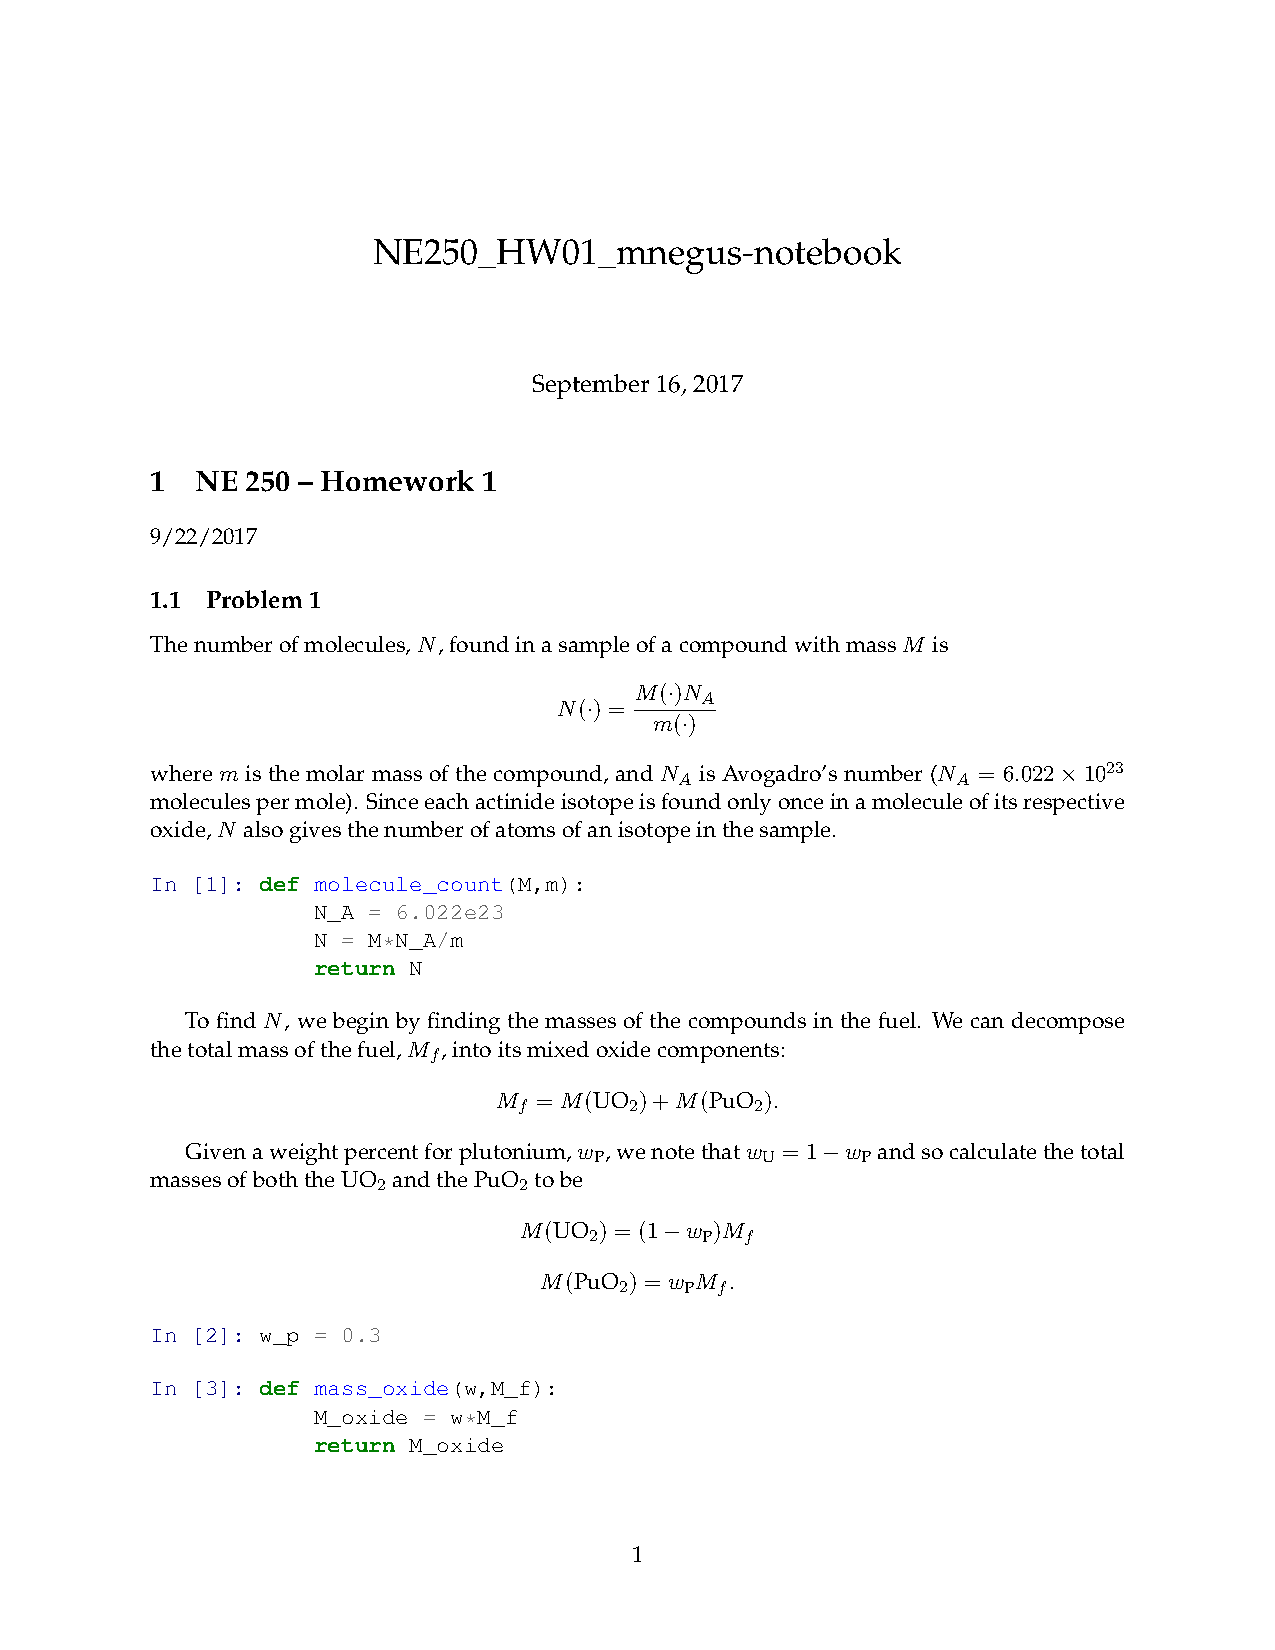
\includepdf[pages=-]{NE250_HW01_mnegus-notebook.pdf}


\end{document}







 